\section{The constant $A(p)$ and the Koenigs obstruction}
\label{sec:ap-koenigs}

Path~C returns to the discrete factor $A(p)$ introduced in Section~\ref{sec:Ap-def}. Path~A already uses $A(p)$ as a well-defined limit, and already notes that, unlike its continuous counterpart $A_{\mathrm{ct}}$, it is not given by a comparably elementary closed formula. The present section makes that statement precise enough for thesis work: we record usable representations, note the numerical and near-critical difficulties, and sketch why an elementary closed form in $p$ is not expected, via the logistic map and its Koenigs linearisation. The heavier conjugacy arguments sit in Appendix~\ref{app:c-koenigs}.

Earlier optimism in the project---that a tidy elementary expression for $A(p)$ might still turn up---is revised here. What replaces it is stronger and more useful: $A(p)$ is computable, has an infinite-product form, admits asymptotics as $p\to\tfrac12^{-}$, and is tied to a classical object in one-dimensional dynamics for which elementary closed forms are known only outside the parameter range relevant to subcritical branching.

\subsection{Recap: definition and conditional mean}
\label{sec:ap-recap}

For the death-or-division Galton--Watson process with division probability $p\in\bigl[0,\tfrac12\bigr)$,
\[
S_{n+1} = 2p\,S_n - p\,S_n^2,
\qquad
S_0=1,
\]
and
\begin{equation}
A(p)
=
\lim_{n\to\infty}
\frac{S_n}{(2p)^n}
\in
\bigl(0,\tfrac12\bigr],
\end{equation}
so that
\[
\lim_{n\to\infty}
\mean{\zz_n\mid \zz_n\neq 0}
=
\frac{1}{A(p)}.
\]
Every analytic question about the limiting conditional mean is therefore a question about $A(p)$.

\subsection{Numerical evaluation}
\label{sec:ap-numeric}

For fixed $p$ bounded away from $\tfrac12$, iteration of the survival recurrence quickly drives $S_n$ into the linear regime $S_{n+1}\approx 2p\,S_n$, so forming the ratio $S_n/(2p)^n$ for large $n$ estimates $A(p)$ to arbitrary precision. The same computation yields the curve of $A(p)$ against $p$ already compared with $A_{\mathrm{ct}}$ in Figure~\ref{fig:dtctA}.

The method degrades as $p\to\tfrac12^{-}$: $A(p)\to 0$, the conditional mean diverges, and the number of generations needed before $S_n$ is small becomes impractically large. Near criticality one therefore needs an asymptotic surrogate (Section~\ref{sec:ap-asymp}) rather than raw iteration alone.

\subsection{Infinite product}
\label{sec:ap-product}

A change of scale places the survival map in logistic form. Set $S_n=2w_n$ and $r=2p\in[0,1)$. Then
\[
w_{n+1} = r\, w_n(1-w_n),
\qquad
w_0=\tfrac12,
\]
which is the logistic map $f_r(w)=r w(1-w)$ on the unit interval. Since
\[
A(p)
=
2\lim_{n\to\infty}\frac{w_n}{r^n},
\]
writing the limit as an infinite product of successive ratios $w_{k+1}/(r w_k)$ yields
\begin{equation}
\label{eq:prodFormula}
A(p)
=
\frac12
\prod_{k=1}^{\infty}
\bigl(1-w_k\bigr)
=
\frac12
\prod_{k=1}^{\infty}
\Bigl(1-\frac{S_k}{2}\Bigr).
\end{equation}
The product converges for $r\in(0,1)$: the inequality $w_{n+1}<r w_n$ implies geometric decay of $w_n$, hence summability of $\sum w_k$ and convergence of $\prod(1-w_k)$. Formula~\eqref{eq:prodFormula} is an exact representation rather than a closed elementary expression, since evaluating it still requires the orbit $(w_k)$ generated by $f_r$. Its value is conceptual---it exhibits $A(p)$ as a functional of the logistic orbit---and computational, as an alternative running product alongside $S_n/(2p)^n$.

\begin{figure}[ht]
\centering
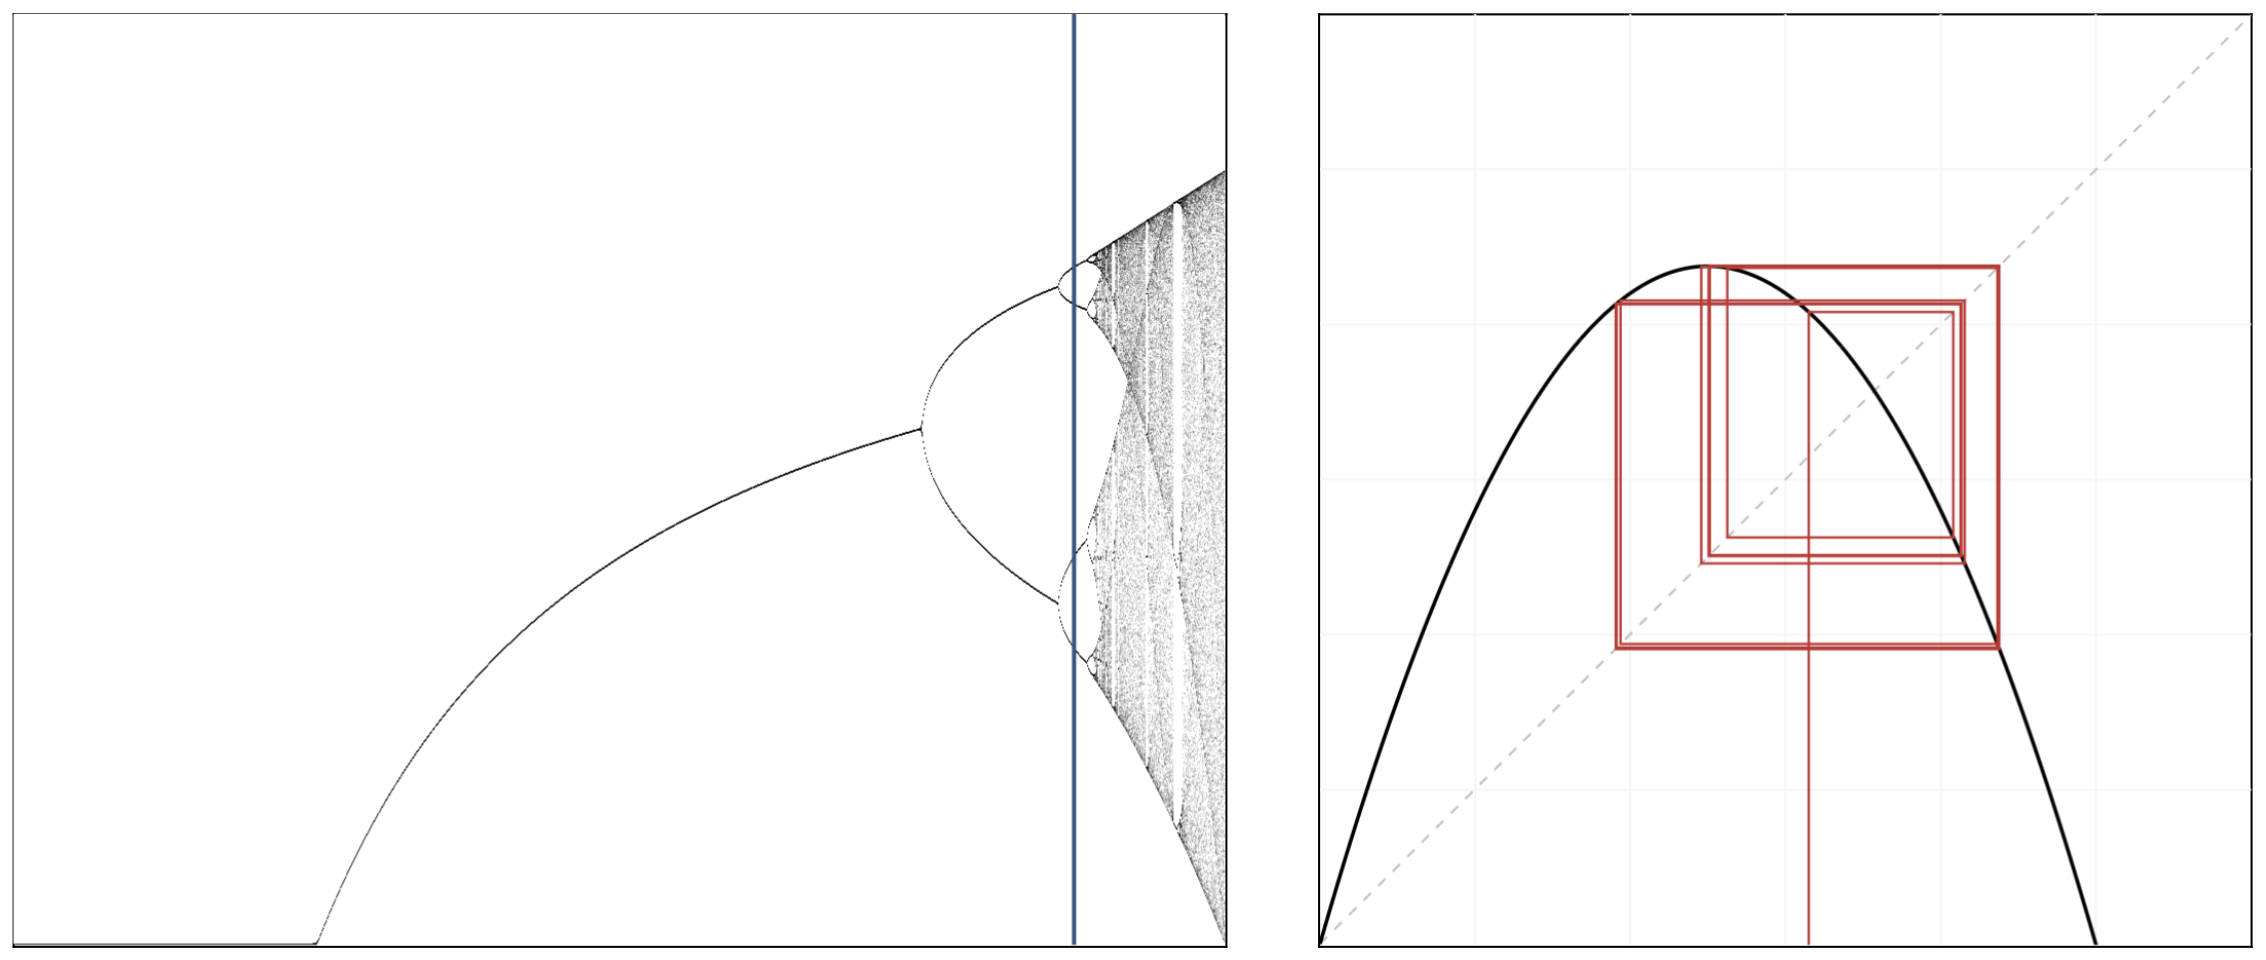
\includegraphics[width=0.75\textwidth]{figures/fig_ap_koenigs/period_double.png}
\caption{The logistic family $f_r(w)=rw(1-w)$ for $r\in[0,4]$ exhibits the familiar period-doubling cascade. Subcritical branching uses only the window $r=2p\in[0,1)$, far below the onset of chaos, but the same map appears in the product formula for $A(p)$.}
\label{fig:logistic-bifurcation}
\end{figure}

\subsection{Asymptotics near criticality}
\label{sec:ap-asymp}

Let $\varepsilon=1-2p\to 0^{+}$, so that $p=\tfrac12(1-\varepsilon)$ approaches criticality from below. The survival recurrence rearranges to
\[
S_{n+1}-S_n
=
(2p-1)S_n - p S_n^2
=
-\varepsilon S_n - \tfrac12 S_n^2 + \tfrac{\varepsilon}{2}S_n^2.
\]
Treating $n$ as continuous for large $n$ and dropping the higher-order term $\varepsilon S_n^2$ produces the approximate ODE
\begin{equation}
\label{eq:S-ode}
\frac{\dd S}{\dd n}
=
-\varepsilon S - \tfrac12 S^2.
\end{equation}
This Riccati equation is elementary. With $u=1/S$ one obtains the linear ODE $u'-\varepsilon u=\tfrac12$; matching $S_0=1$ and the late-time linearisation $S_n\sim A(p)(2p)^n$ then yields the leading near-critical behaviour
\begin{equation}
\label{eq:Ap-asymp}
A(p)
\sim
2\,\varepsilon
=
2(1-2p)
\qquad\text{as }p\to\tfrac12^{-}.
\end{equation}
Consequently
\[
\frac{1}{A(p)}
\sim
\frac{1}{2(1-2p)}
\to\infty
\qquad\text{as }p\to\tfrac12^{-},
\]
which agrees \emph{exactly} at leading order with the continuous picture $1/A_{\mathrm{ct}}=(1-p)/(1-2p)\sim 1/(2(1-2p))$ as $p\to\tfrac12^{-}$. Formula~\eqref{eq:Ap-asymp} thus restores numerical access to $A(p)$ in precisely the window where direct iteration of $S_n$ stalls.

\subsection{Search attempts}
\label{sec:ap-search}

Before the dynamical connection below was appreciated, a natural question was whether $A(p)$ might still be a simple combination of elementary functions of $p$. Direct attacks included continuum ODE approximations of the recurrence and, more experimentally, symbolic regression / genetic search for a closed expression fitted to numerical samples of $A(p)$ (cf.\ the genetic-algorithm experiments archived with the chapter materials). No satisfactory elementary candidate survived. Interactive illustrations of those searches are intended to be linked from the compiled PDF once hosted
% TODO: HTML URL for GA solver
(\texttt{<URL: GA / symbolic regression demo>}).
The negative outcome is consistent with---but weaker than---the Koenigs obstruction of the next subsections: failure to find a formula is not a proof, though it correctly predicted that the object is not elementary in $p$.

\subsection{Logistic map and the Koenigs function}
\label{sec:koenigs-intro}

The substitution $S_n=2w_n$, $r=2p$ has already placed $A(p)$ inside the orbit of the logistic map $f_r$. Koenigs' classical linearisation theorem supplies a change of coordinates that straightens $f_r$ near the attracting fixed point at the origin when $0<|r|<1$ \cite{Koenigs1884}. There exists a unique local holomorphic map $\phi_r$, with $\phi_r(0)=0$ and $\phi_r'(0)=1$, satisfying the Schr\"oder equation
\begin{equation}
\label{eq:schroder}
\phi_r\bigl(f_r(z)\bigr)
=
r\,\phi_r(z)
\end{equation}
in a neighbourhood of $0$. Equivalently,
\begin{equation}
\label{eq:koenigs-limit}
\phi_r(z)
=
\lim_{n\to\infty}
r^{-n} f_r^{\circ n}(z),
\end{equation}
the limit existing uniformly on a neighbourhood of the origin.

\begin{figure}[ht]
\centering
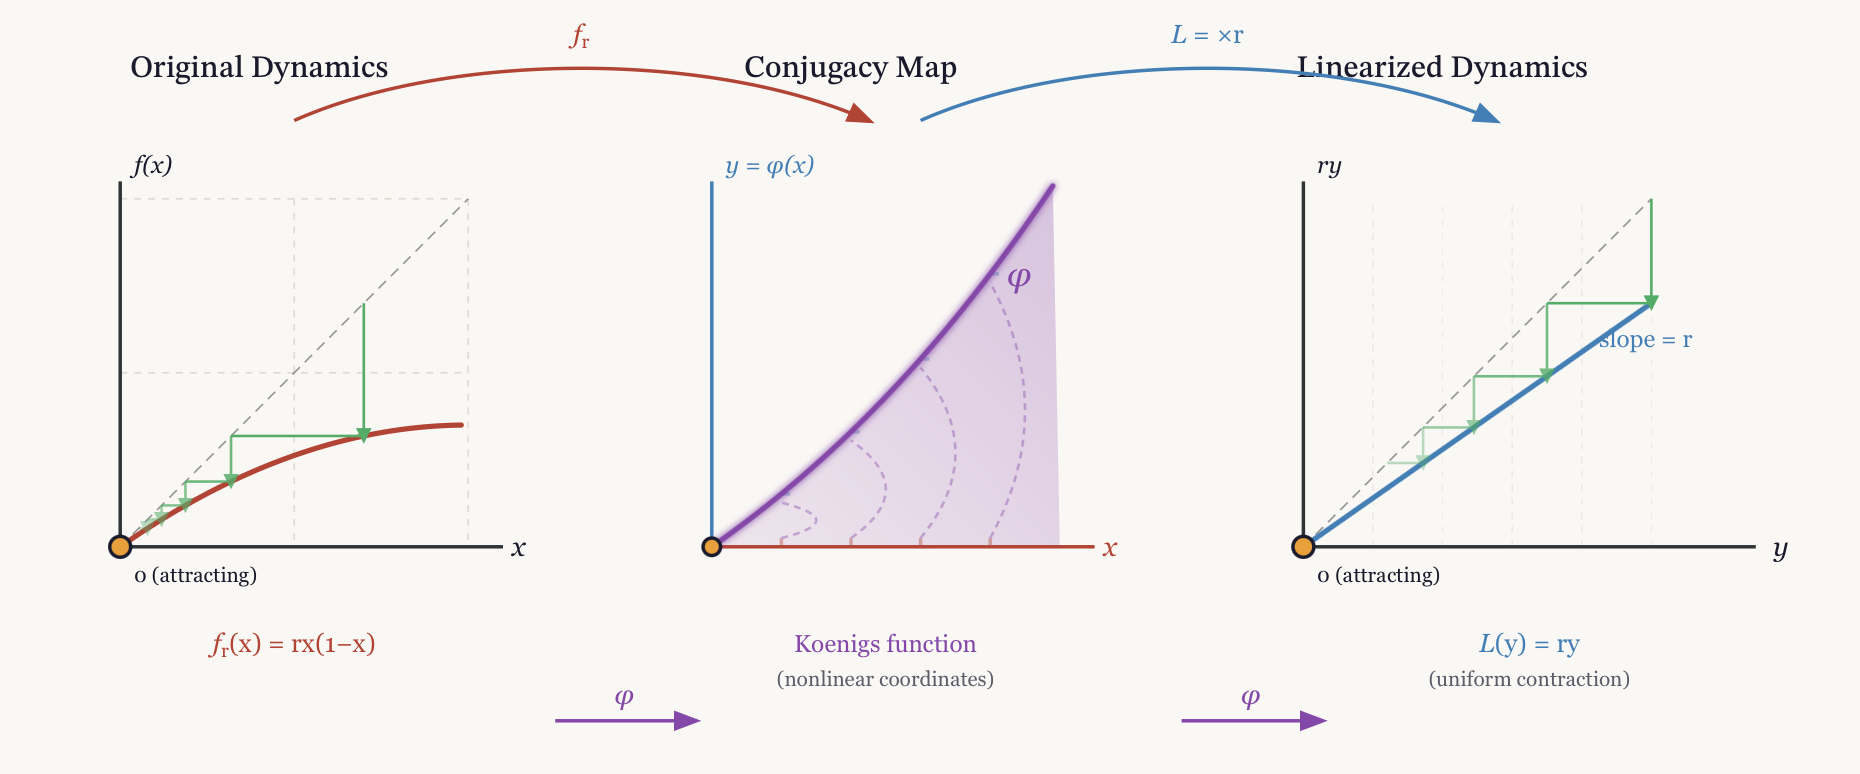
\includegraphics[width=0.75\textwidth]{figures/fig_ap_koenigs/figure2_koenigs_linearization.png}
\caption{Schematic of Koenigs linearisation: the nonlinear logistic map $f_r$ is conjugate, via $\phi_r$, to multiplication by the multiplier $r$ near the origin.}
\label{fig:koenigs-schematic}
\end{figure}

Comparing \eqref{eq:koenigs-limit} with $A(p)=2\lim w_n/r^n$ and $w_{n}=f_r^{\circ n}(w_0)$, $w_0=\tfrac12$, one obtains the structural identity
\begin{equation}
\label{eq:Ap-koenigs}
A(p)
=
2\,\phi_{r}\bigl(\tfrac12\bigr)
\qquad\text{with }r=2p\in[0,1),
\end{equation}
interpreted in the sense of analytic continuation / the global real orbit on $(0,1)$ under the attracting dynamics at $0$ (the point $w_0=\tfrac12$ lies in the real basin for $r\in(0,1)$; details and domain caveats are recorded in Appendix~\ref{app:c-koenigs}). So $A(p)$ is not an arbitrary special function of $p$: it is twice the \emph{basin} Koenigs value $\lim r^{-n}f_r^{\circ n}(\tfrac12)$ (not a naive power-series evaluation outside the local disc), with multiplier $r=2p$.

\subsection{Why an elementary closed form is not expected}
\label{sec:no-elementary}

For each fixed multiplier $r\in(0,1)$, the map $f_r$ is a quadratic rational map with an attracting fixed point at $0$ whose multiplier is not a root of unity. A theorem of Becker and Bergweiler \cite{Becker1995} implies that the Koenigs linearisation of a rational map of degree at least two satisfies an algebraic differential equation if and only if the map is, up to analytic conjugacy, a monomial or Chebyshev map. For the quadratic family those exceptional cases correspond to logistic parameters $r=2$ and $r=4$ (Appendix~\ref{app:c-koenigs}), both \emph{outside} the interval $r\in(0,1)$ relevant to subcritical branching.

For each fixed $p\in\bigl(0,\tfrac12\bigr)$, then, the linearisation of the associated logistic map is non-elementary as a function of its spatial argument, in the sense made precise in Appendix~\ref{app:c-koenigs} (hypertranscendence of the conjugacy for multipliers in $(0,1)$, with the classical elementary logistic cases $r=2$ and $r=4$ lying outside that interval). Extracting $A(p)$ from that conjugacy therefore cannot proceed by evaluating a single elementary expression for the conjugacy as a function of $z$.

\paragraph{Honest scope of the claim.}
Two logical gaps remain if one wants a theorem stronger than the working claim below. First, non-elementarity of a function $z\mapsto\phi(z)$ does not by itself forbid a closed form for a single value $\phi(\tfrac12)$ (compare $\Gamma$ and $\Gamma(\tfrac12)=\sqrt{\pi}$); results on transcendency of \emph{values} of local conjugacies would be needed to close that gap. Second, passing from fixed-$r$ statements to a classification of the scalar map $p\mapsto A(p)$ is a further step. We do not claim either completion here. The working thesis claim, sufficient for applications and for revising the earlier ``still attainable'' hope, is:

\begin{quote}
\textit{No elementary closed-form expression for $A(p)$ on $p\in[0,\tfrac12)$ is known, and none is expected: $A(p)$ is tied to the linearisation of the logistic map at multiplier $r=2p\in[0,1)$, in a regime where that conjugacy is non-elementary for each fixed $r\in(0,1)$, while the classical elementary logistic cases $r=2,4$ lie outside the subcritical branching range.}
\end{quote}

In that sense Path~A's punchline stands, Path~C supplies mechanism and partial theorem, and $A(p)$ remains a perfectly usable numerical and asymptotic object.

\begin{figure}[ht]
\centering
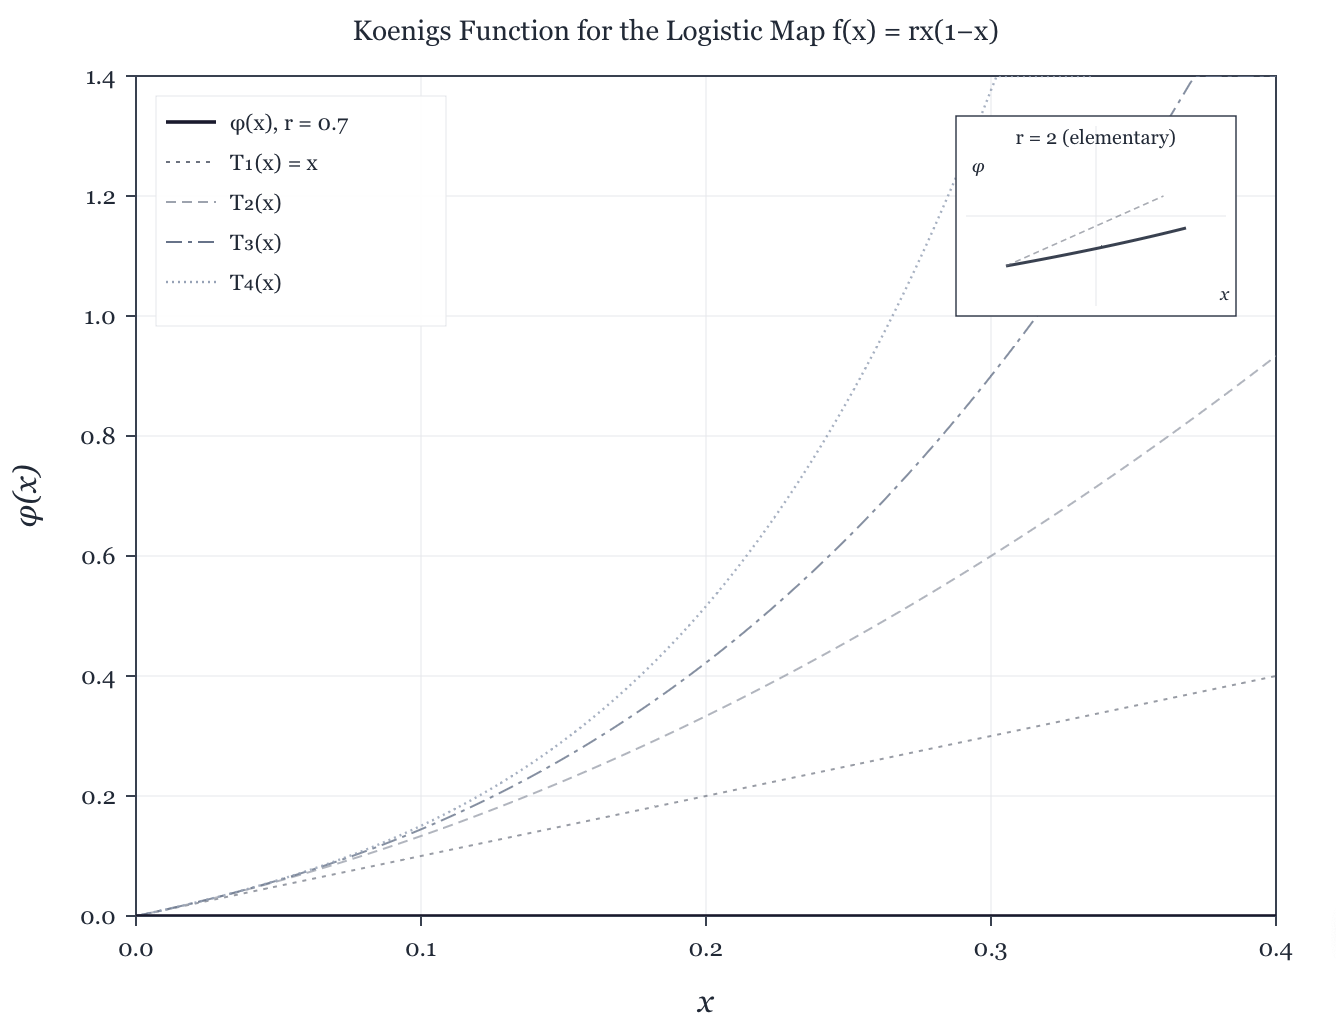
\includegraphics[width=0.7\textwidth]{figures/fig_ap_koenigs/figure3_numerical_koenigs.png}
\caption{Numerical approximation of a Koenigs function for a logistic multiplier in $(0,1)$, together with low-order Taylor polynomials near the origin. The conjugacy is smooth but not polynomial; elementary closed forms are available only for exceptional multipliers outside this range.}
\label{fig:koenigs-numeric}
\end{figure}

\paragraph{Fractal aside.}
In the complex plane the same Koenigs conjugacies organise the local dynamics of quadratic maps whose global Julia sets are fractal. That geometric picture explains, informally, why one should not expect a simple elementary formula for the linearisation---but it is scenery, not a substitute for the Becker--Bergweiler dichotomy above.

\subsection{Usable conclusions for the thesis}
\label{sec:ap-takeaway}

For the rest of the thesis one may treat $A(p)$ as:
\begin{enumerate}[leftmargin=*]
\item well defined by \eqref{eq:Ap-limit} for each $p\in\bigl[0,\tfrac12\bigr)$;
\item computable by iteration or by the product \eqref{eq:prodFormula}, with asymptotics \eqref{eq:Ap-asymp} near criticality;
\item the reciprocal of the discrete quasi-stationary mean, in parallel with elementary $A_{\mathrm{ct}}$ in continuous time;
\item not replaceable, in the subcritical binary model, by a known elementary closed form in $p$.
\end{enumerate}

\subsection*{Close of the chapter}

Path~A fixed the Markov, branching, and quasi-stationary language used throughout the thesis, including the continuous elementary counterpart of $A(p)$ and the sensitivity of survival to small founding cohorts. Path~B developed the characteristic method for the continuous-time absorption generating functions used later in BDC analysis. Path~C completed the discrete story of $A(p)$: representation, numerics, near-critical asymptotics, and a Koenigs-based account of why an elementary formula should not be expected. The appendices hold the heavier algebra. What remains for later chapters is application---not a missing elementary expression for $A(p)$.
